\documentclass{mythesis}

\usetikzlibrary{decorations.markings}
\usepackage{pgfplots}
\pgfplotsset{compat=1.11}

\DeclareDocumentCommand{\Ind}{}{\operatorname{Ind}}

\ExplSyntaxOn
\DeclareDocumentCommand { \Index } { lmg } {
    \IfNoValueTF { #1 } {
        { [ #2 : #3 ] }
    } {
        \mathopen{[} #2 \mathbin{:} #3 \mathclose{] #1}
    }
}
\ExplSyntaxOff


\title{Der reell-algebraische Abbildungsgrad}
\author{Stephan Hilb}

\begin{document}

\maketitle

\begin{abstract}
    Die Windungszahl einer polynomiellen Kurve $\gamma: [0, 1] \to \C^*$ lässt sich als halben Cauchy-Index der rationalen Funktion $\frac{\Re \gamma}{\Im \gamma}$ auf $[0,1]$ definieren, was anschaulich gesprochen die Überquerungen der Kurve an der rellen Achse mit $\pm \frac{1}{2}$ zählt.
    Ein reell-algebraischer Algorithmus, basierend auf polynomieller Restbildung oder sogenannten Sturm-Ketten, erlaubt die explizite Berechnung dieses Cauchy-Index und damit auch der Windungszahl von $\gamma$.

    Nach einer Einführung werden wir einen ähnlichen Algorithmus für den Abbildungsgrad, der Verallgemeinerung der Windungszahl in höheren Dimensionen, formulieren und untersuchen.
\end{abstract}


{\let\clearpage\relax\tableofcontents}


\section{Der univariate Fall, Windungszahl und Cauchy-Index}

\subsection{Geometrische Motivation}

Die Windungszahl einer geschlossenen Kurve $\gamma: [a,b] \to \C^*$ bezeichnet die Anzahl der entgegen dem Uhrzeigersinn gerichteten\footnote{ein rechtshändig orientiertes kartesisches Koordinatensystem vorausgesetzt} Umläufe von $\gamma$ um die $0$.
Dies lässt sich am leichtesten visuell in Abbildung \ref{fig:winding_number} nachvollziehen.

\begin{figure}[ht]
    \centering
    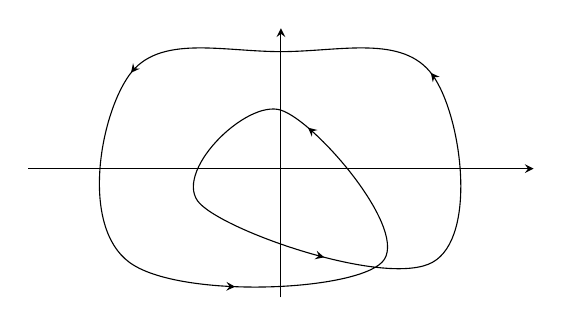
\begin{tikzpicture}
        \begin{axis}[
            height=5cm,
            width=8cm,
            axis x line=middle,
            axis y line=middle,
            xmin=-2.5,xmax=2.5,
            ymin=-1.1,ymax=1.2,
            ticks=none,
        ]
            \addplot[smooth cycle,tension=0.7,
                postaction={decorate},
                decoration={markings,
                    mark=at position 0.1 with {\arrow{stealth}},
                    mark=at position 0.3 with {\arrow{stealth}},
                    mark=at position 0.5 with {\arrow{stealth}},
                    mark=at position 0.7 with {\arrow{stealth}},
                    mark=at position 0.9 with {\arrow{stealth}},
                }
            ] coordinates
                { (1.5,0.8) (0,1.0) (-1.5,0.8) (-1.5,-0.8) (1,-0.8) (0,0.5) (-0.8,-0.3) (1.5,-0.8) };
        \end{axis}
    \end{tikzpicture}
    \caption{Kurve mit Windungszahl 2}
    \label{fig:winding_number}
\end{figure}

Formalisieren lässt sich die Windungszahl auf viele verschiedene Arten und Weisen.
Eine traditionelle Idee für die Formalisierung ist das Aufsummieren der Winkel, die beim Durchlaufen der Kurve mit dem Ursprung eingeschlossen werden.
Die Topologie stellt beispielsweise simpliziale Approximation wie in \cite[§I1f,§I1h]{eiserm_topology} bereit, um die Winkelzählung auf eine endliche Summation zu reduzieren.
Im Analysis-Werk \cite[§12.7]{koenigsberger1} wird der Begriff der \emph{Liftung} eingeführt, um die Winkeländerung zu erfassen.
Abgesehen davon hat die Windungszahl auch eine Integraldarstellung $\frac{1}{2\pi i} \int_{\gamma} \frac{1}{z} \di[z]$, die in der komplexen Analysis sehr gebräuchlich ist.
%Siehe dazu beispielsweise \cite{??}.

In unseren Anwendungen werden wir uns auf stückweise polynomielle Kurven beschränken und können daher eine einfachere und zugleich intuitive Definition wählen.

Eine polynomielle Kurve $\gamma: [a,b] \to \C^*$ besteht aus polynomiellem Realteil $p := \Re \gamma$ und polynomiellem Imaginärteil $q := \Im \gamma$.
Für $p,q \neq 0$ sind daher insbesondere die Anzahl Schnittpunkte von $\gamma$ mit der imaginären, bzw. der reellen Achse endlich.
Wir nutzen dies, um die Übergänge der Kurve an der reellen Achse wie in Abbildung \ref{fig:curve_counting_full} zu zählen und anschließend aufzusummieren.

\begin{figure}[ht]
    \centering
    \begin{subfigure}[t]{0.49\textwidth}
        \centering
        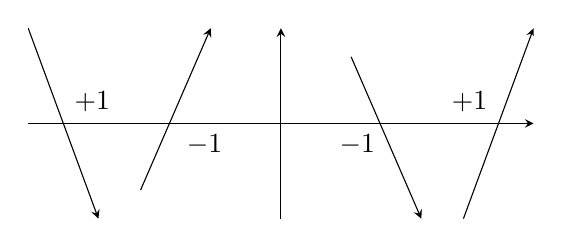
\begin{tikzpicture}[>=stealth,label distance=-0.15cm]
            \begin{axis}[
                height=4cm,
                width=8cm,
                axis y line=middle,
                axis x line=middle,
                ticks=none,
            ]
                \addplot[->] coordinates
                    { (-1.8,1) (-1.3,-1) };
                    \node[label=above right:{$+1$}] at (axis cs:-1.55,0) {};
                \addplot[->] coordinates
                    { (-1,-0.7) (-0.5,1) };
                    \node[label=below right:{$-1$}] at (axis cs:-0.75,0) {};
                \addplot[->] coordinates
                    { (0.5,0.7) (1,-1) };
                    \node[label=below left:{$-1$}] at (axis cs:0.75,0) {};
                \addplot[->] coordinates
                    { (1.3,-1) (1.8,1) };
                    \node[label=above left:{$+1$}] at (axis cs:1.55,0) {};
            \end{axis}
        \end{tikzpicture}
        \caption{Vollständige Übergänge}
        \label{fig:curve_counting_full}
    \end{subfigure}
    \begin{subfigure}[t]{0.49\textwidth}
        \centering
        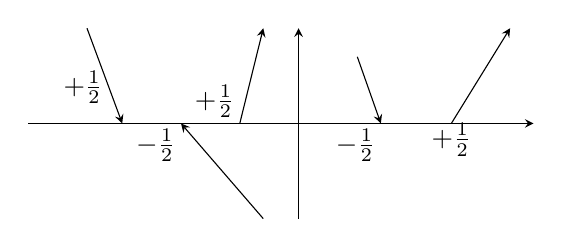
\begin{tikzpicture}[>=stealth,label distance=-0.25cm]
            \begin{axis}[
                height=4cm,
                width=8cm,
                axis y line=middle,
                axis x line=middle,
                ticks=none,
                xmin=-2.3,
                xmax=2.0
            ]
                \addplot[->] coordinates
                    { (-1.8,1) (-1.5,0) };
                    \node[label={[label distance=0cm]above left:{$+\frac{1}{2}$}}] at (axis cs:-1.5,0) {};
                \addplot[->] coordinates
                    { (-0.3,-1) (-1,0) };
                    \node[label=below left:{$-\frac{1}{2}$}] at (axis cs:-1,0) {};
                \addplot[->] coordinates
                    { (-0.5,0) (-0.3,1) };
                    \node[label=above left:{$+\frac{1}{2}$}] at (axis cs:-0.5,0) {};
                \addplot[->] coordinates
                    { (0.5,0.7) (0.7,0) };
                    \node[label=below left:{$-\frac{1}{2}$}] at (axis cs:0.7,0) {};
                \addplot[->] coordinates
                    { (1.3,0) (1.8,1) };
                    \node[label=below:{$+\frac{1}{2}$}] at (axis cs:1.3,0) {};
            \end{axis}
        \end{tikzpicture}
        \caption{Halbe Übergänge}
        \label{fig:curve_counting_half}
    \end{subfigure}
    \caption{Zählen von Achsenübergängen}
    \label{fig:curve_counting}
\end{figure}

Da wir uns bei der Zählung nicht auf geschlossene Kurven beschränken wollen, nutzen wir die Konvention aus \ref{fig:curve_counting_half}, um auch Übergänge von Kurven zu erfassen, die auf der reellen Achse starten, bzw. enden.
Hiermit stellen wir die Subdivisionseigenschaft sicher, welche später ausgeführt wird (siehe \ref{thm:cauchy-index_properties}).

Die so erhaltene Zählung der Achsenübergänge nennen wir \emphdef{Cauchy-Index} und schreiben dafür $\Ind_a^b(p : q)$.
Für die Windungszahl ergibt sich damit
\begin{math}
    \deg(\gamma) = \frac{1}{2} \Ind_a^b(p : q).
\end{math}
Mit anderen Worten: zählen wir die Übergänge an der reellen Achse wie in Abbildung \ref{fig:curve_counting}, so ergibt sich die Windungszahl gerade als die Hälfte dessen.

Wir werden den Cauchy-Index nun formalisieren.

\begin{definition}[Cauchy-Index] \label{thm:df:cauchy_index}
    Seien $p, q \in \R[X]$ reelle Polynome ohne gemeinsame Nullstellen und $a, b \in \R$ mit $a \le b$.
    Für jede Nullstelle $s \in \R$ von $q$, d.h. $q(s) = 0$, sei $\epsilon > 0$ hinreichend klein, dass $\sgn\big(q(t)\big)$ jeweils auf $[s - \epsilon, s)$ und $(s, s + \epsilon]$ konstant ist.

    Wir definieren nun
    \begin{math}
        \Ind_s^{\pm}(p:q) &:= \begin{cases}
            \frac{1}{2} \sgn\big(p(s)\big) \sgn\big(q(s \pm \epsilon)\big) & \text{für $q(s) = 0$}, \\
            0 & \text{sonst},
        \end{cases}\\
        \Ind_s(p:q) &:= \Ind_s^+(p:q) - \Ind_s^-(p:q), \\
        \Ind_a^b(p:q) &:= \Ind_a^+(p:q) + \sum_{s \in (a,b)} \Ind_s(p:q) - \Ind_b^-(p:q).
    \end{math}
    $\Ind_a^b(p:q)$ nennen wir \emphdef[Cauchy-Index]{Cauchy-Index von $p$ und $q$ auf $[a,b]$}.
\end{definition}

\begin{note}
    \begin{itemize}
        \item
            Die Definition ist offenbar unabhängig von der Wahl von $\epsilon$.
        \item
            Die Summe $\sum_{s\in (a,b)} \Ind_s(p:q)$ ist wohldefiniert, da $\Ind_s(p:q)$ nur an endlich vielen Stellen einen Beitrag leistet.
        \item
            Im Fall $q = \const$ oder $p = 0$ erhält man sofort $\Ind_s(p:q) = 0$.
        %\item
        %    $\Ind_s(p:q)$ zählt den Übergang der Kurve $\gamma(t) = p(t) + iq(t)$ an der reellen Achse in $t = s$, wie bereits in \ref{fig:curve_counting} veranschaulicht.
        \item
            In der Literatur (beispielsweise in \cite[Definition 6.27]{linalg_ratapprox_orthpoly} wird der Cauchy-Index auf $[a,b]$ auch anhand der Polstellen der rationalen Funktion $r = \frac{p}{q}$ auf $[a,b]$ definiert:
            \begin{math}
                I_s(r) &:= \begin{cases}
                    1 & \lim_{x \nearrow s} r(x) = -\infty \land \lim_{x \searrow s} r(x) = \infty, \\
                    -1 & \lim_{x \nearrow s} r(x) = \infty \land \lim_{x \searrow s} r(x) = -\infty, \\
                    0 & \text{sonst},
                \end{cases}\\
                I_a^b(r) &:= \sum_{s \in [a,b]} I_s(r)
            \end{math}
            Polstellen von $r$ in $a$ und $b$ werden hierbei oft ausgeschlossen.
            Es ist leicht nachvollziehbar, dass unter dieser Annahme beide Definitionen übereinstimmen.

            Die Randterme $\Ind_a^+$, $\Ind_b^-$ mit dem Faktor $\frac{1}{2}$ in unserer Definition \ref{thm:df:cauchy_index} erlauben es, der Einschränkung an den Rändern auf geschickter Weise zu entkommen, ohne dabei auf die typischen Eigenschaften des Cauchy-Index (siehe \ref{thm:cauchy-index_properties}) verzichten zu müssen.
    \end{itemize}
\end{note}

\begin{example}
    Sei $p \in \R[x]$, $a,b \in \R$ mit $a < b$ und $p$ besitze nur einfache Nullstellen.
    Wir können den Cauchy-Index nutzen, um die Nullstellen von $p$ in $(a,b)$ zu zählen:
    Der Cauchy-Index $\Ind_a^b(p':p)$ zählt die Anzahl der Nullstellen von $p$ in $[a,b]$, Nullstellen auf dem Rand $\Set{a,b}$ werden mit dem Gewicht $\frac{1}{2}$ gezählt.

    \begin{proof}
        Es ist leicht einzusehen, dass an jeder (einfachen) Nullstelle $x \in \R$ von $p$ gilt $\sgn(p'(x)) = \pm\sgn(p(x\pm\nobreak\eps))$ mit $\eps$ hinreichend klein, dass $p$ auf $[x-\eps,x)$, bzw. $(x,x+\eps]$ konstantes Vorzeichen hat.
        Damit folgt direkt
        \begin{math}
            \Ind_a^\pm(p':p) = \begin{cases}
                \pm \frac{1}{2} & p(x) = 0 \\
                0 & p(x) \neq 0
            \end{cases}
        \end{math}
        und die Behauptung folgt.
    \end{proof}
\end{example}

%Im Folgenden seien $p, q \in \R[x]$ solange nicht anderweitig festgelegt stets reelle Polynome ohne gemeinsame Nullstellen.
Es bietet sich an, die Definition zu verallgemeinern.
Wir werden später sehen, dass dies in der Tat auch sinnvoll ist.

\begin{definition}
    Seien $p, q: \R \to \R$ stückweise polynomielle, reelle Funktionen ohne gemeinsame Nullstellen und $a, b \in \R$.

    Für $a < b$ definieren den Cauchy-Index $\Ind_a^b(p:q)$ wie in \ref{thm:df:cauchy_index}.
    Für $a > b$ fordern wir \emphdef{Antisymmetrie}: $\Ind_a^b(p:q) := -\Ind_b^a(p:q)$ und für $a = b$ setzen wir $\Ind_a^b(p:q) := 0$.
\end{definition}

Der Cauchy-Index entspricht auch in der erweiterten Fassung unserer Intuition.
Beispielsweise zählt $\Ind_a^b(p:\nobreak q)$ für $a > b$ die Achsenübergänge auf $[b, a]$ in umgekehrter Durchlaufrichtung.

%
%
%\begin{tikzpicture}
%    \begin{axis}
%        \addplot[samples=100,domain=-1:1]({2*x^2 - 1}, {x^3 - x});
%    \end{axis}
%\end{tikzpicture}



\subsection{Eigenschaften des Cauchy-Index}

\begin{proposition}[Eigenschaften] \label{thm:cauchy-index_properties}
    Seien $p, q, s: \R \to \R$ stückweise polynomielle, reelle Funktionen und $a, b, c \in \R$.
    Weiter seien $p, q$ ohne gemeinsame Nullstellen.
    Der Cauchy-Index genügt folgenden Eigenschaften:
    \begin{enumerate}[i)]
        \item
            \emph{Subdivision}: $\Ind_a^b(p:q) = \Ind_a^c(p:q) + \Ind_c^b(p:q)$,
        \item
            \emph{Homogenität}: $\sgn(c) \Ind_a^b(p:q) = \Ind_a^b(cp:q) = \Ind_a^b(p:cq)$,
        \item
            \emph{Invarianz unter Transformation}: für $\tau: \R \to \R$ stückweise polynomiell und streng monoton auf $[a, b]$, bzw. $[b, a]$ gilt
            \begin{math}[numbered] \label{eq:cauchy-index_transformation}
                \Ind_a^b(p\circ\tau : q\circ\tau) = \Ind_{\tau(a)}^{\tau(b)}(p:q),
            \end{math}
        \item
            \emph{Scherung}: $\Ind_a^b(p:q) = \Ind_a^b(p + sq : q)$,
        \item
            \emph{Inversion}: $\Ind_a^b(p:q) + \Ind_a^b(q:p) = \Ind_a^b(1:pq)$,
        \item
            \emph{Reduktion}: $\Ind_a^b(1:q) = \frac{1}{2}\big(\sgn(q(b)) - \sgn(q(a))\big)$.
    \end{enumerate}
    \begin{note}
        Während die Eigenschaften i)-iii) praktisch für spätere Beweisführungen sind, werden uns vor allem iv)-vi) erlauben, den Cauchy-Index algorithmisch zu bestimmen.
    \end{note}
    \begin{proof}
        \begin{enumerate}[i)]
            \item
                Wegen $\Ind_a^b(p:q) = -\Ind_b^a(p:q)$ genügt es den Fall $a \le c \le b$ zu betrachten, alle anderen Fälle können durch Umbenennung der Variablen in diesen überführt werden.
                Die Fälle in denen Gleichheit zwischen $a$, $b$ oder $c$ auftritt sind trivial wegen $\Ind_a^a(p:q) = 0$.
                Sei also $a < c < b$, dann gilt
                \begin{math}
                    &\Ind_a^c(p:q) + \Ind_c^b(p:q) \\
                    &\quad = \Ind_a^+(p:q) + \sum_{s\in(a,c)}\Ind_s(p:q) \underbrace{- \Ind_c^-(p:q) + \Ind_c^+(p:q)}_{=\Ind_c(p:q)} + \sum_{s\in(c,b)} \Ind_s(p:q) - \Ind_b^-(p:q) \\
                    &\quad = \Ind_a^b(p:q).
                \end{math}
            \item
                Es genügt wieder den Fall $a < b$ zu betrachten.
                Für $c = 0$ ist die Aussage trivial.
                Für $c > 0$ ändern sich bei der Multiplikation von $p$, bzw. $q$ mit $c$ keine Vorzeichen, also $\Ind_a^b(p:q) = \Ind_a^b(cp:\nobreak q) = \Ind_a^b(p:cq)$.
                Für $c < 0$ kehren sich entsprechend die Vorzeichen in der Definition um, also $\Ind_a^b(cp:\nobreak q) = - \Ind_a^b(p:q) = \Ind_a^b(p:q)$.
            \item
                Sei wieder ohne Einschränkung $a < b$.
                Betrachte zunächst $\tau(x) := b+a-x$: an den Nullstellen $s$ von $q\circ \tau$ gilt offenbar $\Ind_s^\pm(p\circ\tau : q\circ\tau) = \Ind_{\tau(s)}^\mp(p:q)$ und damit
                \begin{math}
                    \Ind_a^b(p\circ\tau : q\circ\tau) = -\Ind_b^a(p : q).
                \end{math}
                Sei $\tau$ nun streng monoton fallend, so ist $\hat \tau(x) := \tau(b + a - x)$ streng monoton steigend und es gilt
                \begin{math}
                    \Ind_a^b(p\circ \tau : q \circ \tau) &= - \Ind_a^b(p \circ \hat \tau : q \circ \hat \tau), \\
                    \Ind_{\tau(a)}^{\tau(b)}(p:q) &= - \Ind_{\hat\tau(a)}^{\hat\tau(b)}(p:q).
                \end{math}
                Es genügt also, im folgenden $\tau$ als streng monoton steigend vorauszusetzen.

                Da $\tau$ das Intervall $[a,b]$ bijektiv auf $[\tau(a), \tau(b)]$ abbildet, können wir für beide Seiten der Gleichung \eqref{eq:cauchy-index_transformation} Subdivision derart anwenden, dass beide Intervalle in die selbe Anzahl Teilintervalle zerlegt werden und in jedem Paar von Teilintervallen $q\circ \tau$ und $q$ jeweils genau eine Nullstelle besitzen.
                Durch weitere Subdivision und Antisymmetrie können wir sogar annehmen, dass diese Nullstellen stets am linken Rand $a$ angenommen werden.

                Intervalle ohne solche Nullstellen leisten keinen Beitrag in \eqref{eq:cauchy-index_transformation} und können ignoriert werden.
                Für alle anderen Intervalle gilt am linken Endpunkt mit der Wahl $\delta := \tau(a + \epsilon) - \tau(a)$ wegen Monotonie von $\tau$
                \begin{math}
                    \Ind_a^+(p\circ \tau : q \circ \tau)
                    &= \frac{1}{2}\sgn\big(p(\tau(a))\big) \sgn\big(q(\tau(a+\epsilon))\big) \\
                    &= \frac{1}{2}\sgn\big(p(\tau(a))\big) \sgn\big(q(\tau(a) + \delta)\big) \\
                    &= \Ind_{\tau(a)}^+(p : q)
                \end{math}
                und somit $\Ind_a^b(p \circ \tau : q \circ \tau) = \Ind_{\tau(a)}^{\tau(b)}(p:q)$.
            \item
                Zunächst ist klar, dass auch $p + sq$ und $q$ keine gemeinsamen Nullstellen besitzen.
                Mit der selben Technik wie im Beweis von iii) genügt es jetzt $\Ind_a^+(p:q) = \Ind_a^+(p+sq:q)$ zu zeigen.
                Dies ist jedoch leicht einzusehen, da $\sgn(p(a)) = \sgn\big((p+sq)(a)\big)$ wenn $q$ in $a$ eine Nullstelle besitzt.
            \item
                Es genügt mittels Subdivision und Transformation den Term $\Ind_a^+(1:pq)$ zu betrachten, wobei $a$ Nullstelle von $pq$ ist.
                Sei ohne Einschränkung $a$ Nullstelle von $q$, also insbesondere $p(a) \neq 0$.
                Dann gilt
                \begin{math}
                    \Ind_a^+(1:pq)
                    &= \frac{1}{2} \sgn\big((pq)(a+\epsilon)\big) \\
                    &= \frac{1}{2} \sgn(p(a)) \sgn(q(a+\epsilon)) \\
                    &= \Ind_a^+(p:q) + \Ind_a^+(q:p),
                \end{math}
                da $pq$ auf $(a, a+\epsilon]$ konstantes Vorzeichen hat und somit auch $p$ auf $[a, a + \epsilon]$.
            \item
                Die rechte Seite erfüllt offenbar ebenfalls Antisymmetrie und Subdivision.
                Es genügt also wieder, die Gleichheit für $\Ind_a^+(1:q)$ zu zeigen, wobei $a$ Nullstelle von $q$ ist.
                So gilt
                \begin{math}
                    \Ind_a^+(1:q)
                    = \frac{1}{2} \sgn(q(a+\epsilon))
                    = \frac{1}{2} \big(\sgn(q(b)) - \sgn(q(a))\big),
                \end{math}
                denn die Wahl $\epsilon := b - a$ ist legitim.
        \end{enumerate}
    \end{proof}
\end{proposition}


\subsection{Berechenbarkeit}


Wie bereits versprochen konstruieren wir uns nun mit Hilfe obiger Eigenschaften den folgenden Algorithmus.

\begin{algorithm} \label{thm:cauchy-index_simple}
    \Input{$p,q \in \R[x]$ ohne gemeinsame Nullstellen, $a,b \in \R$} \\
    \Output{$\Index_a^b{p}{q} = \Ind_a^b(p:q)$}
    \begin{algorithmic}[1]
        \If{$p = \const$}
            \Return{$\frac{1}{2} \sgn(p) \big(\sgn(q(b)) - \sgn(q(a))\big)$}
        \Else
            \State{bestimme $s,r \in \R[x]$ so, dass $p = sq - r$ mit $\deg r < \deg q$} \Comment{z.B. durch Polynomdivision}
            \Return{$\Index_a^b{q}{r} - \Index_a^b{1}{qr}$}
        \EndIf
    \end{algorithmic}
\end{algorithm}

\begin{proposition}
    Algorithmus \ref{thm:cauchy-index_simple} terminiert und berechnet ein korrektes Ergebnis.
    \begin{proof}
        Betrachte den rekursiven Aufruf von $\Index_a^b{q}{r}$ in Zeile 5.
        Falls $\deg p \le \deg q$, so ist nun $\deg q > \deg r$ für den nächsten Schritt der Rekursion.
        Falls $\deg p > \deg q$, so erfolgt der nächste Aufruf mit geringerem Grad für $p$.
        Nach endlich vielen Schritten terminiert also die Rekursion.

        Im Fall $p = \const$ (Zeile 2) liefert Homogenität und Reduktion aus \ref{thm:cauchy-index_properties} direkt
        \begin{math}
            \Ind_a^b(p:q) = \frac{1}{2} \sgn(p) \big(\sgn(q(b)) - \sgn(q(a)\big).
        \end{math}
        Falls $p \neq \const$ (Zeilen 4-5) ist wegen $p = sq - r$ mittels Scherung, Homogenität und Inversion
        \begin{math}
            \Ind_a^b(p:q) = \Ind_a^b(sq - r: q)
            = -\Ind_a^b(r : q)
            = \Ind_a^b(q : r) - \Ind_a^b(1 : qr).
        \end{math}
        Die Rekursion führt somit zu einem korrekten Ergebnis.
    \end{proof}
\end{proposition}

Wir betrachten erneut Algorithmus \ref{thm:cauchy-index_simple} und beobachten, dass durch die Rekursion Aufrufe der Form $\Index_a^b{p_0}{p_1},\allowbreak \Index_a^b{p_1}{p_2}, \dotsc, \Index_a^b{p_{n-1}}{p_n}$ entstehen.
Hierbei ist $(p_0, \dotsc, p_n)$ eine Kette von Polynomen, welche durch die Polynom-Rest-Bildung $p_{k-1} = s_kp_k - p_{k+1}$ entsteht.
Wir nennen eine solche Kette auch \emphdef{euklidische Kette}.

Für eine solche Kette gilt stets
\begin{math}
    \Index_a^b{p_{k-1}}{p_k}
    = -\Index_a^b{p_{k+1}}{p_k}
    = \Index_a^b{p_k}{p_{k+1}} - \Index_a^b{1}{p_kp_{k+1}}.
\end{math}
Nutzen wir dies und erstellen eine Kette mit der Wahl $p_0 := q, p_1 := p$, so erhalten wir
\begin{math}
    \Index_a^b{p}{q}
    = \Index_a^b{p_1}{p_0}
    &= \Index_a^b{1}{p_0p_1} - \Index_a^b{p_0}{p_1} \\
    &= \Index_a^b{1}{p_0p_1} + \Index_a^b{1}{p_1p_2} - \Index_a^b{p_1}{p_2} \\
    &= \dotsc \\
    &= \sum_{k=1}^n \Index_a^b{1}{p_{k-1}p_k} - \Index_a^b{p_{n-1}}{p_n}.
\end{math}
Der letzte Term entfällt, falls $p_n$ konstant ist und wir können die Berechnung des Cauchy-Index auch wie folgt formulieren.

\begin{algorithm} \label{thm:cauchy-index_premseq}
    \Input{$p,q \in \R[x]$ ohne gemeinsame Nullstellen, $a,b \in \R$} \\
    \Output{$\Index_a^b{p}{q} = \Ind_a^b(p:q)$}
    \begin{algorithmic}[1]
        \If{$p = 1$}
            \Return{$\frac{1}{2} \big(\sgn(q(b)) - \sgn(q(a))\big)$}
        \Else
            \State{bestimme eine euklidische Kette $(p_0, p_1, \dotsc, p_n)$ mit $p_0 := q, p_1 := p$}
            \Return{$\sum_{k=1}^n \Index_a^b{1}{p_{k-1}p_k}$}
        \EndIf
    \end{algorithmic}
\end{algorithm}

Diese Formulierung wird unser Vorbild sein, wenn wir im nächsten Kapitel den bivariaten Fall behandeln.


\subsection{Sturm-Ketten}


\begin{definition}
    Sei $s_0, \dotsc, s_n \in \R[x]$ und $a,b \in \R, a \le b$.
    Die Sequenz $(s_0, \dotsc, s_n)$ von reellen Polynomen heißt \emphdef{Sturm-Kette bezüglich $[a,b]$}, falls
    \begin{enumerate}[i)]
        \item
            $\forall x \in [a,b], 0 < k < n: s_k(x) = 0 \implies s_{k-1}(x) s_{k+1}(x) < 0$,
        \item
            $\sgn(s_n(x)) = \const$ auf $[a,b]$.
    \end{enumerate}
    \begin{note}
        In einer Sturm-Kette besitzen insbesondere je zwei Nachbarn $p_{k-1}, p_k$ keine gemeinsamen Nullstellen.
    \end{note}
\end{definition}

\begin{example}
    Seien $p_0, p_1 \in \R[x]$ ohne gemeinsame Nullstellen.
    Die euklidische Kette $(p_0, p_1, \dotsc, p_n)$ ist eine Sturm-Kette.
    \begin{proof}
        Seien $p_{k-1}, p_k$ ohne gemeinsame Nullstellen.
        Dann ist für alle $x \in \R$ mit $p_k(x) = 0$
        \begin{math}
            0 \neq p_{k-1}(x)
            = s(x) p_k(x) - p_{k+1}(x)
            = - p_{k+1}(x).
        \end{math}
        Folglich haben $p_k$ und $p_{k+1}$ ebenfalls keine gemeinsamen Nullstellen und es gilt $p_{k-1}(x) p_{k+1}(x) < 0$ an allen Nullstellen $x$ von $p_k$.
        Induktiv ergibt sich zusammen mit $\deg(p_n) = 0$ die Behauptung.
    \end{proof}
\end{example}

\begin{lemma} \label{thm:sturm_boundary-terms}
    Für eine Sturm-Kette $(s_0, \dotsc, s_n)$ gilt
    \begin{math}[numbered] \label{eq:sturm_boundary-terms}
        \Index_a^b{s_1}{s_0}
        = \sum_{k=1}^n \Index_a^b{1}{s_{k-1}s_k}.
    \end{math}
    \begin{proof}
        $s_{k-1}$ und $s_{k+1}$ besitzen an den Nullstellen von $s_k$ jeweils verschiedene Vorzeichen.
        Wir erhalten also durch Einfügen von Summanden der Form $\Index_a^b{s_{k-1}}{s_k} + \Index_a^b{s_{k+1}}{s_k} = 0$
        \begin{math}
            \Index_a^b{s_1}{s_0}
            &= \Index_a^b{s_1}{s_0} + \Index_a^b{s_{n-1}}{s_n} \\
            &= \sum_{k=1}^n \Big( \Index_a^b{s_k}{s_{k-1}} + \Index_a^b{s_{k-1}}{s_k} \Big)
            = \sum_{k=1}^n \Index_a^b{1}{s_{k-1}s_k}.
        \end{math}
    \end{proof}
\end{lemma}

Wir werden die rechte Seite in \eqref{eq:sturm_boundary-terms} in Form von Vorzeichenwechsel beschreiben.

\begin{definition}
    Für $a_0, \dotsc, a_n \in \R$ definieren wir die \emphdef{Anzahl von Vorzeichenwechsel}
    \begin{math}
        V(a_0, \dotsc, a_n) :=
        \sum_{k=1}^n \frac{1}{2} \big|\sgn(a_{k-1}) - \sgn(a_k)\big|.
    \end{math}
    Wir nutzen für eine Kette von Polynomen $p_0, \dotsc, p_n \in \R[x]$ und $a, b \in \R$ die Notation
    \begin{math}
        V_a^b(p_0, \dotsc, p_n) := V\big(p_0(a), \dotsc, p_n(a)\big) - V\big(p_0(b), \dotsc, p_n(b)\big).
    \end{math}
\end{definition}


\begin{theorem}[Sturm, Cauchy]
    Seien $p, q \in \R[x]$ Polynome ohne gemeinsame Nullstellen.
    Weiter sei $(s_0, \dotsc, s_n)$ eine Sturm-Kette mit $s_0 = q, s_1 = p$.
    Dann gilt
    \begin{math}
        \Index_a^b{p}{q}
        = V_a^b(s_0, \dotsc, s_n).
    \end{math}
    \begin{proof}
        $s_{k-1}, s_k$ besitzen keine gemeinsamen Nullstellen.
        Ohne Einschränkung erhalten wir also durch Multiplikation mit $|\sgn(s_{k-1}(x))| = 1$
        \begin{math}
            \big|\sgn(s_{k-1}(x)) - \sgn(s_k(x))\big|
            = \big|1 - \sgn\big((s_{k-1}s_k)(x)\big) \big|
            = 1 - \sgn\big((s_{k-1}s_k)(x)\big)
        \end{math}
        und somit dank Reduktion aus \ref{thm:cauchy-index_properties}
        \begin{math}
            V_a^b(s_{k-1},s_k)
            &= \frac{1}{2} \Big( 1 - \sgn\big((s_{k-1}s_k)(b)\big) \Big)
              - \frac{1}{2} \Big( 1 - \sgn\big((s_{k-1}s_k)(a)\big) \Big) \\
            &= \Index_a^b{1}{s_{k-1}s_k}.
        \end{math}
        Die Aussage folgt jetzt aus direkt aus \ref{thm:sturm_boundary-terms}:
        \begin{math}
            V_a^b(s_0,\dotsc, s_n)
            = \sum_{k=1}^n V_a^b(s_{k-1}, s_k)
            = \sum_{k=1}^n \Index_a^b{1}{s_{k-1}s_k}
            = \Index_a^b{s_1}{s_0}.
        \end{math}
    \end{proof}
\end{theorem}















\subsection{Geometrische Charakterisierung der Windungszahl}










%\begin{tikzpicture}
%    \begin{axis}
%        \addplot3[surf,faceted color=black,color=red,colormap/greenyellow]({x},{y},{x^2});
%    \end{axis}
%\end{tikzpicture}












\end{document}
